\documentclass[12pt]{article}
\usepackage{greg}
\usepackage[baskerville,vvarbb]{newtxmath}
\usepackage{fontspec}
\usepackage{titlesec}
\usepackage[nottoc]{tocbibind}

\usepackage{fancyvrb}
\setmainfont{Baskerville}
\setsansfont{Quadrat-Serial}
\setmonofont{Courier New}

\titleformat*{\section}{\large\sffamily}
\titleformat*{\subsection}{\normalsize\sffamily}
\titleformat*{\subsubsection}{\normalsize\sffamily}
\titleformat{\chapter}[hang]{\LARGE\sffamily}{\LARGE\thechapter}{1ex}{}[]
\titleformat{name=\chapter,numberless}[hang]{\LARGE\sffamily}{}{0ex}{}[]

\title{Discrete gauge theory in homotopy type theory}
\author{Greg Langmead}
\begin{document}

\begin{abstract}
We identify connections, curvature, and gauge transformations within the structures of homotopy type theory. Whereas most classical treatments of these structures rely entirely on infinitesimal definitions, there is an equivalent discrete story of which the infinitesimal version is a limit, analogous to the relationship between smooth paths and tangent vectors, or between de Rham and Čech cohomology. We will show how to identify the elements of discrete gauge theory, provide some evidence that this is what we have found, and use it to prove some results from the 20th century mathematics of gauge theory that depend only on homotopy types.
\end{abstract}

%\tableofcontents

\section{Introduction}
\begin{quote} 
\centering 
"It is always ourselves we work on, whether we realize it or not. There is no other work to be done in the world." --- Stephen Talbott, \emph{The Future Does Not Compute}\cite{talbott}
\end{quote}

Homotopy type theory (HoTT) is a logical foundation for mathematics that adds to set theory several important mathematical patterns. Among these are \emph{fibrations}, \emph{(higher) groupoids}, and \emph{classifying spaces} (called \emph{universes}). It embodies the philosophy of constructivism by unifying mathematical statements with types and proofs with terms. It has an extensive syntax and a talented team of theory builders who have labored for a decade to equip the syntax with formal initiality proofs and categorical semantics that together generate living, breathing proofs simultaneously in every category with enough structure to support the semantics. It has implementations in several computer languages which have attracted multiple large formalization efforts. It benefits from an unusually strong interdisciplinary culture spanning computer science, mathematics, philosophy, and physics.

The hypothetical scope of HoTT is of course all of mathematics, past, present and future. It contains set theory, and the law of excluded middle and axiom of choice can be added whenever the intended semantics supports them. It therefore invites us to use the rest of its tools to enhance our understanding, and to seek better answers to \emph{why} questions in the same way that category theory sometimes tells us \emph{why} individual results across specific fields are true. Over the last decade many results have been verified in HoTT, and many have insightful new proofs. The topics that have received the most attention so far include homotopy theory, algebraic topology, group theory, category theory, and combinatorics. Our goal is to extend this list with topics from geometry: connections, curvature, gauge theory, characteristic classes, and Chern-Weil theory.

Gauge theory is a collection of tools inspired by, and in dialog with, the standard model of particle physics. The quantum field theories developed during the 20th century are mathematical models that supply spacetime with additional structures: principal bundles, vector bundles, sections of these bundles, and connections. The bundles provide internal dimensions to quantum particles, which are visible experimentally through phenomena such as charge, magnetism, mass, gravity, and quark color. Forces are mediated by massless particles that correspond to the connections. Particles are sections of associated vector bundles. Physical laws are expressed by real- or complex-valued functions called lagrangians, on the configuration space of all of this structure.

Mathematicians discovered that by adding their own gauge theory structures to smooth manifolds of interest they could define new invariants of the homotopy type, the homeomorphism class, or the diffeomorphism class of the manifold. HoTT is not equipped today to explore all of these scenarios since it is most developed in the world of homotopy types only. There is beautiful work to bring in notions of topology and smooth structure through the principal of \emph{cohesion} (the study of spatial relationships by way of operators that \emph{remove} such structure). We will touch on some of this and point the way to future work, but for now we will focus on homotopical results only. 

For the HoTT-oriented audience my goal is to demonstrate that connections and gauge theory are present in the realm of discrete types. This can even serve as an introduction to classical differential geometry, and today's undergraduates who are drawn to HoTT can leverage their intuitions to bypass a lot of confusing material!

For the geometry audience my goal is to offer an entirely new perspective on the de Rham complex in general, and connections and curvature in particular. My grandiose hope is that in this framing we can find a natural and intuitive understanding of Chern-Weil theory, i.e. the link between curvature and characteristic classes. 


\section{Non-infinitesimal calculus}

Our plan is to examine differential geometry using finite methods: using paths instead of vector fields. We will apply the syntax of type theory and work through a first course in differential forms, connections and curvature.

We will use a heuristic to guide us: whenever a classical statement uses infinitesimal objects we should find an equivalent one that uses finite objects. We should try to restate results involving tangent vectors using finite-length paths instead. We should try to replace 1-forms with integrals of the 1-form over paths.

In addition to changing our perspective on classical geometry we will make a concession on the type theory side: we will work with objects in HoTT that are \emph{discrete}, meaning devoid of cohesion or spatial information. Manifolds will be combinatorial objects, not based on the real numbers. There are three consolations for this loss: first, we will still have access to results in gauge theory that depend only on the homotopy type. Secondly we can approximate a curved manifold as closely as we want by adding more points, paths, and so on to the mesh, bringing more use cases into our construction. And lastly we will hopefully gain a lot of insight into the inner workings of classical differential geometry.

Classically, functions on the level of points such as a smooth function between smooth manifolds \( f:M\to N \) can be differentiated to yield a new function that acts on both points and tangent vectors: \( Tf:TM\to TN \). There is no new data in \( Tf \), its action on vectors is computed in terms of its action on points. We package the derived (no pun) data into a new function that acts on both points and vectors. Passing through the heuristic we proposed, we would instead package the derived information as the action on finite-length paths in \( M \). Tangent vectors are equivalence classes of such paths anyway, so it seems no information is lost. This would mean that taking the derivative of a smooth function is the same as to extract its action on paths.

The derivative is a particular action on paths, one that is entailed in the original function on points. Classically the derivative can be pulled apart to examine \emph{only} its action on paths, often called \( df \). This is a 1-form, meaning a section of the cotangent bundle. A 1-form is an object defined on all of \( M \) which can be integrated over a path to give a number. Again, a function on paths. An arbitrary 1-form is some function on paths, and \( df \) is one such.

HoTT also has functions, but those functions always act in all the available dimensions of the type all at once. It is inherently a function on points, paths, and higher paths. We can look at what \( f \) does to paths using the construction \( \ap f \). At this point there is an important check we can make. \( df \) has a few important properties, the most characteristic of which is the Leibniz, or product rule. Is this visible in HoTT?

The Leibniz rule states that if \( f, g:M\to \rr \) are two smooth functions to the real numbers then \( d(fg) = fdg + gdf \). Here \( fg \) is the function formed by taking the pointwise product of \( f \) and \( g \). To examine this situation in HoTT we need type-theoretic functions \( f, g:M\to B \) from some type \( M \) to an H-space \( B \).

\begin{mydef}
An H-space structure on a pointed type \( (B,b) \) consists of
\begin{enumerate}
\item A binary operation \( \mu:B\to B\to B \)
\item A left unit law \( \mu_l:\mu(\pt,-)=\id_B \)
\item A right unit law \( \mu_r:\mu(-,\pt)=\id_B \)
\item A coherence \( \mu_{lr}:\mu_l(\pt)=_{\mu(\pt,\pt)=\pt}\mu_r(\pt) \)
\item A proof of left- and right- invertibility: \( \mu(a,-):A\simeq A \), \( \mu(-, b):A\simeq A \)
\end{enumerate}
\end{mydef}

The analogue of the algebra of functions to \( \rr \) is:
\begin{myprop}
For any type \( M \) and H-space \( B \) the type of maps \( M\to B \) with base point the constant map is an H-space under pointwise multiplication.
\end{myprop}

We claim thact the following deserves to be called the Leibniz rule.

\begin{mylemma}
For any type \( M \) and H-space \( B \) and maps \( f,g:M\to B \) and path \( p:x=_M y \) we have \( \ap(fg)(p)=\mu(f(x),\ap(g)(p)) \cdot \mu(\ap(f)(p),g(y)) \). (\( \cdot \) is concatenation of paths.)
\end{mylemma}

The notation is temporarily sloppy, but by \( \mu(a, p) \) for a path \( p \) we mean the functorial action of multiplication by \( a \) on the left, on a path.g

% https://q.uiver.app/#q=WzAsMyxbMCwwLCJCIl0sWzEsMCwiQiJdLFsyLDAsIkIiXSxbMCwxLCJcXG11KGEsLSkiLDAseyJjdXJ2ZSI6LTJ9XSxbMCwxLCJcXG11KGEnLC0pIiwyLHsiY3VydmUiOjJ9XSxbMSwyLCJcXG11KC0sYikiLDAseyJjdXJ2ZSI6LTJ9XSxbMSwyLCJcXG11KC0sYicpIiwyLHsiY3VydmUiOjJ9XSxbMyw0LCJwIiwyLHsic2hvcnRlbiI6eyJzb3VyY2UiOjIwLCJ0YXJnZXQiOjIwfX1dLFs1LDYsInEiLDIseyJzaG9ydGVuIjp7InNvdXJjZSI6MjAsInRhcmdldCI6MjB9fV1d
\begin{tikzcd}[cramped]
  B & B & B
  \arrow[""{name=0, anchor=center, inner sep=0}, "{\mu(a,-)}", curve={height=-12pt}, from=1-1, to=1-2]
  \arrow[""{name=1, anchor=center, inner sep=0}, "{\mu(a',-)}"', curve={height=12pt}, from=1-1, to=1-2]
  \arrow[""{name=2, anchor=center, inner sep=0}, "{\mu(-,b)}", curve={height=-12pt}, from=1-2, to=1-3]
  \arrow[""{name=3, anchor=center, inner sep=0}, "{\mu(-,b')}"', curve={height=12pt}, from=1-2, to=1-3]
  \arrow["p"', shorten <=3pt, shorten >=3pt, Rightarrow, from=0, to=1]
  \arrow["q"', shorten <=3pt, shorten >=3pt, Rightarrow, from=2, to=3]
\end{tikzcd}

\begin{figure}[h]
\centering
\begin{tikzpicture}[
node distance = 15mm and 15mm,
V/.style = {circle, fill, draw=black, inner sep=1pt, font=\footnotesize},
every edge quotes/.style = {auto, font=\footnotesize},
arrow/.style={->,semithick}
]
\begin{scope}[nodes=V]
  \node[label=above left:\( b \)] (1) {};
  \node[label=above right:\( r \)] (2) [right=of 1]  {};
  \node[label=below right:\( g \)] (3) [below=of 2]  {};
  \node[label=below left:\( o \)] (4) [below=of 1]  {};
\end{scope}
\draw[arrow]
        (1)  edge["\( br \)"] (2)
        (2)  edge["\( rg \)"] (3)
        (3)  edge["\( go \)"] (4)
        (4)  edge["\( ob \)"] (1);
\end{tikzpicture}
\caption{The HIT \( C_4 \) which is one of the types in \( \BAutoso \)}
\end{figure}

\begin{figure}[h]
\centering
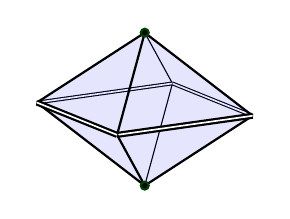
\begin{tikzpicture}%
  [x={(-0.860769cm, -0.121512cm)},
  y={(0.508996cm, -0.205391cm)},
  z={(-0.000053cm, 0.971107cm)},
  scale=1,
  back/.style={thin},
  dim2back/.style={double, thin},
  edge/.style={black, thick},
  dim2edge/.style={black, double, thick},
  facet/.style={fill=blue!95!black,fill opacity=0.1},
  vertex/.style={inner sep=1pt,circle,draw=green!25!black,fill=black,thick},
  dim1vertex/.style={}]
\coordinate (-1, -1, 0) at (-1, -1, 0);
\coordinate (-1, 1, 0) at (-1, 1, 0);
\coordinate (0, 0, -1) at (0, 0, -1);
\coordinate (0, 0, 1) at (0, 0, 1);
\coordinate (1, -1, 0) at (1, -1, 0);
\coordinate (1, 1, 0) at (1, 1, 0);
%% Drawing edges in the back
%%
\draw[edge,dim2back] (-1, -1, 0) -- (-1, 1, 0);
\draw[edge,back] (-1, -1, 0) -- (0, 0, -1);
\draw[edge,back] (-1, -1, 0) -- (0, 0, 1);
\draw[edge,dim2back] (-1, -1, 0) -- (1, -1, 0);
%% Drawing vertices in the back
%%
\node[dim1vertex] at (-1, -1, 0)     {};
%% Drawing the facets
%%
\fill[facet] (1, 1, 0) -- (0, 0, -1) -- (1, -1, 0) -- cycle {};
\fill[facet] (1, 1, 0) -- (0, 0, 1) -- (1, -1, 0) -- cycle {};
\fill[facet] (1, 1, 0) -- (-1, 1, 0) -- (0, 0, 1) -- cycle {};
\fill[facet] (1, 1, 0) -- (-1, 1, 0) -- (0, 0, -1) -- cycle {};
%% Drawing edges in the front
%%
\draw[edge] (-1, 1, 0) -- (0, 0, -1);
\draw[edge] (-1, 1, 0) -- (0, 0, 1);
\draw[dim2edge] (-1, 1, 0) -- (1, 1, 0);
\draw[edge] (0, 0, -1) -- (1, -1, 0);
\draw[edge] (0, 0, -1) -- (1, 1, 0);
\draw[edge] (0, 0, 1) -- (1, -1, 0);
\draw[edge] (0, 0, 1) -- (1, 1, 0);
\draw[dim2edge] (1, -1, 0) -- (1, 1, 0);
%% Drawing the vertices in the front
%%
\node[dim1vertex] at (-1, 1, 0)     {};
\node[vertex] at (0, 0, -1)     {};
\node[vertex] at (0, 0, 1)     {};
\node[dim1vertex] at (1, -1, 0)     {};
\node[dim1vertex] at (1, 1, 0)     {};
\end{tikzpicture}
\caption{The HIT \( \Sigma C_4 \) which has 2 points, 4 1-paths, 4 2-paths.}
\end{figure}

\begin{figure}[h]
\centering
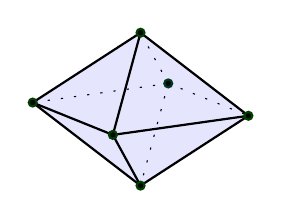
\begin{tikzpicture}%
  [x={(-0.860769cm, -0.121512cm)},
  y={(0.508996cm, -0.205391cm)},
  z={(-0.000053cm, 0.971107cm)},
  scale=1,
  back/.style={loosely dotted, thin},
  edge/.style={black, thick},
  facet/.style={fill=blue!95!black,fill opacity=0.1},
  vertex/.style={inner sep=1pt,circle,draw=green!25!black,fill=black,thick}]
\coordinate (-1, -1, 0) at (-1, -1, 0);
\coordinate (-1, 1, 0) at (-1, 1, 0);
\coordinate (0, 0, -1) at (0, 0, -1);
\coordinate (0, 0, 1) at (0, 0, 1);
\coordinate (1, -1, 0) at (1, -1, 0);
\coordinate (1, 1, 0) at (1, 1, 0);
%% Drawing edges in the back
%%
\draw[edge,back] (-1, -1, 0) -- (-1, 1, 0);
\draw[edge,back] (-1, -1, 0) -- (0, 0, -1);
\draw[edge,back] (-1, -1, 0) -- (0, 0, 1);
\draw[edge,back] (-1, -1, 0) -- (1, -1, 0);
%% Drawing vertices in the back
%%
\node[vertex] at (-1, -1, 0)     {};
%% Drawing the facets
%%
\fill[facet] (1, 1, 0) -- (0, 0, -1) -- (1, -1, 0) -- cycle {};
\fill[facet] (1, 1, 0) -- (0, 0, 1) -- (1, -1, 0) -- cycle {};
\fill[facet] (1, 1, 0) -- (-1, 1, 0) -- (0, 0, 1) -- cycle {};
\fill[facet] (1, 1, 0) -- (-1, 1, 0) -- (0, 0, -1) -- cycle {};
%% Drawing edges in the front
%%
\draw[edge] (-1, 1, 0) -- (0, 0, -1);
\draw[edge] (-1, 1, 0) -- (0, 0, 1);
\draw[edge] (-1, 1, 0) -- (1, 1, 0);
\draw[edge] (0, 0, -1) -- (1, -1, 0);
\draw[edge] (0, 0, -1) -- (1, 1, 0);
\draw[edge] (0, 0, 1) -- (1, -1, 0);
\draw[edge] (0, 0, 1) -- (1, 1, 0);
\draw[edge] (1, -1, 0) -- (1, 1, 0);
%% Drawing the vertices in the front
%%
\node[vertex] at (-1, 1, 0)     {};
\node[vertex] at (0, 0, -1)     {};
\node[vertex] at (0, 0, 1)     {};
\node[vertex] at (1, -1, 0)     {};
\node[vertex] at (1, 1, 0)     {};
\end{tikzpicture}
\caption{The HIT \( \{w, y\}* C_4 \) which has 6 points, 12 1-paths, 8 2-paths.}
\end{figure}

\section{The tangent bundle of the 2-sphere}

The classical 2-sphere embedded in \( \rr^3 \) is curved at every point. But we can quantize this curvature by integrating it over a triangulation. Consider two great circles at 90 degree angles to each other, passing through the north and south pole, and take the equator. Convert this data into a combinatorial structure:

\begin{enumerate}
\item The set of vertices \( \{w, y, b, g, r, o, y\} \) where \( w \) is the north pole, \( y \) the south pole, and around the equator are the points of intersection of the three circles, labeled in eastward order \( \{b, o, g, r\} \). The names come from the colors on a standard Rubik's cube.
\item The set of edges generated by the direct paths between adjacent vertices, denoted \( \{wb\}, \{wo\}  \) and so on.
\item The set of faces generated by the triangular regions bounded by three vertices and three paths, denoted \( \{wbo\}, \{wog\} \) and so on.
\end{enumerate}

Parallel transport in the tangent bundle around the \( \{wog\} \) face will rotate a tangent vector by 90 degrees clockwise. This is true for all the triangular faces and so the sum of the action of all 8 faces will be two rotations around the circle. We can compare this result to the standard smooth Gauss-Bonnet theorem.

We can leverage the syntax of HoTT by encoding the above in a map between HITs.

\begin{mydef}
Denote by \( C_4 \) the join \( \{b, g\}*\{r, o\} \). This is the equator of the discrete octahedral sphere. Denote by \( \oo \) the octahedron given by the join \( \{w, y\}* C_4 \).
\end{mydef}

\begin{mylemma}
\( (C_4, b)\equiv S^1 \).
\end{mylemma}

\begin{mylemma}
\( \oo\equiv S^2 \).
\end{mylemma}

\begin{mydef}
Let \( \BAutoso\defeq \sit{X:\U}||X=S^1||_0. \)
\end{mydef}

\begin{mylemma}
We have \( (C_4, ||\{b, g, r, o\}\mapsto \mathsf{base}, br\mapsto \mathsf{loop}, \{rg, go, ob\}\mapsto \refl ||_0):\BAutoso \)
\end{mylemma}

\begin{mylemma}
\( \BAutoso \) is equivalent to the type of \( S^1 \)-torsors, and to the type of \( (C_4,b) \)-torsors.
\end{mylemma}

We will denote other terms of \( \BAutoso \) with notation like \( [w, o, y, r] \), meaning the square isomorphic to \( C_4 \) but with the given four points, and with pointing given by whichever point we listed first. We will also introduce notation for maps \( f:[a, b, c, d]\to [w, x, y, z] \) by indicating where each item in the domain list is sent, like so: \( f\defeq[[x, y, z, w]] \).

\( C_4 \) has an unpointed automorphism connected to the identiy which will play the role of rotation by 90 degrees:

\begin{mydef}
Let \( R:C_4\to C_4 \) be given by \( R(b)=o, R(o)=g, R(g)=r, R(r)=b, R(bo)=og, R(og)=gr, R(gr)=rb, R(rb)=bo. \) Let \( R':R=\id \) be the obvious homotopy to the identity.
\end{mydef}

\begin{mydef}
Define \( T_1:\oo\to\BAutoso \) by 
\begin{itemize}
\item \( T_1(b)=[w, o, y, r] \) (the equator from the point of view of \( b \) as the north pole).
\item \( T_1(o)=[w, b, y, g] \).
\item \( T_1(g)=[w, r, y, o] \).
\item \( T_1(r)=[w, g, y, b] \).
\item \( T_1(w)=[b, o, g, r] \).
\item \( T_1(y)=[b, r, g, o] \).
\item \( T_1(bo)=[[w, g, y, b]] \) (tipping one equator onto the other).
\item \( T_1(og)=[[w, o, y, r]] \).
\item \( T_1(gr)=[[w, g, y, b]] \).
\item \( T_1(rb)=[[w, r, y, o]] \).
\item \( T_1(wb)=[[y, o, w, r]] \).
\item \( T_1(wo)=[[b, y, g, w]] \).
\item \( T_1(wg)=[[w, o, y, r]] \).
\item \( T_1(wr)=[[b, w, g, y]] \).
\item \( T_1(yb)=[[w, r, y, o]] \).
\item \( T_1(yo)=[[b, y, g, w]] \).
\item \( T_1(yg)=[[y, r, w, o]] \).
\item \( T_1(yr)=[[b, w, g, y]] \).
\end{itemize}
\end{mydef}

At this point we have defined a map on the 1-skeleton of \( \oo \). The only constraint we had to follow was functoriality, that the imgage of 1-paths had to be 1-paths between the images. The choices we made were motivated by the embedding of the Rubik's cube in Euclidean 3-space.

\begin{myclaim}
\( T_1 \) defines a principal circle bundle with connection over the 1-skeleton of \( \oo \).
\end{myclaim}

We now want to extend this map to all of \( \oo \) by providing values for the eight faces. Here we will be guided by the classical relationship between a connection and its curvature. The curvature is computed from the connection, it doesn't contain any new data. Classically the integral of curvature over a 2-cell is the holonomy given by transport around the boundary. Can we make this idea type check?

Take the closed path \( wb\cdot bo\cdot ow \) that begins and ends at \( w \), which bounds the face \( wbo \). We can calculate that \( T_1(wb)\cdot T_1(bo)\cdot T_1(ow) = [[r, b, o, g]] = R \), rotation clockwise one notch. A 2-path would then be a homotopy \( \refl_w=R \) which we called \( R' \). In a similar way all 8 faces (so long as the vertices in its name are listed in clockwise order) map to \( R' \).

This is all classical combinatorial stuff, but in a HoTT package. The fact that \( \BAutoso \) is a 2-type gives us someplace to send all the dimensions of the HIT \( \oo \). 
\bibliography{connections}
\end{document}

